\documentclass[a4paper]{report}
\input{~/Developer/LaTeX-Template/Note/header.tex}
\author{Pingbang Hu}
\title{MATH561/IOE510/TO518\\Linear Programming}

\thispagestyle{empty}
\addbibresource{reference.bib}

\newcommand{\Primal}{\mathrm{P}}
\newcommand{\Dual}{\mathrm{D}}
\newcommand{\Main}{\mathrm{M}}
\newcommand{\Sub}{\mathrm{SUB}}
\newcommand{\CSP}{\mathrm{CSP}}
\newcommand{\LB}{\mathrm{LB}}
\newcommand{\UB}{\mathrm{UB}}
\DeclareMathOperator{\Proj}{Proj}

\begin{document}

\maketitle

\begin{abstract}
	This is the first course in the series of graduate-level, large-scale and rigorous mathematical programming courses taught by \href{https://sites.google.com/site/jonleewebpage/}{Jon Lee} at University of Michigan, and in particular, we will use the book write by professor Lee~\cite{Linear-Opt}. This is a dynamic book which may changes and update constantly. In this course, we focus on developing a rigorous understanding on large-scale linear programming problems and also introduce the basic concept of integer programming.

	\vfill
	\begin{center}
		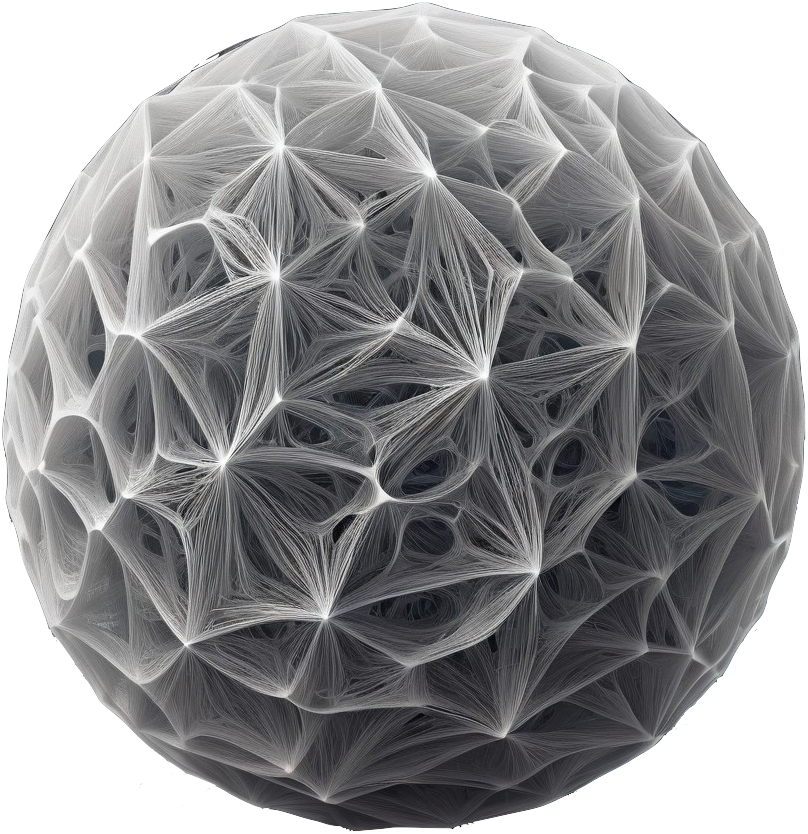
\includegraphics[width=.8\linewidth]{Figures/cover.png}
	\end{center}
	\vfill
	This course is taken in Fall 2021, and the date on the cover page is the last updated time.
\end{abstract}

\tableofcontents

%─────Lectures───────────────────────────────────────────────────────────────────────────────────────────────────────────────────────────────────────
\newpage

\lec{1}{24}

\newpage
%─────Reference──────────────────────────────────────────────────────────────────────────────────────────────────────────────────────────────────────
\pagestyle{plain}
\printbibliography{}

\end{document}